\subsection{Capacitances}
\label{sec:capacitances}

Capacitances between pins of each MOSFET are interesting. They contribute to the potential oscillation circuit, so they should be minimized. The step-by-step method of capacitance extraction is found in Section \ref{sec:extraction}.

\begin{figure}[H]
	\centering
	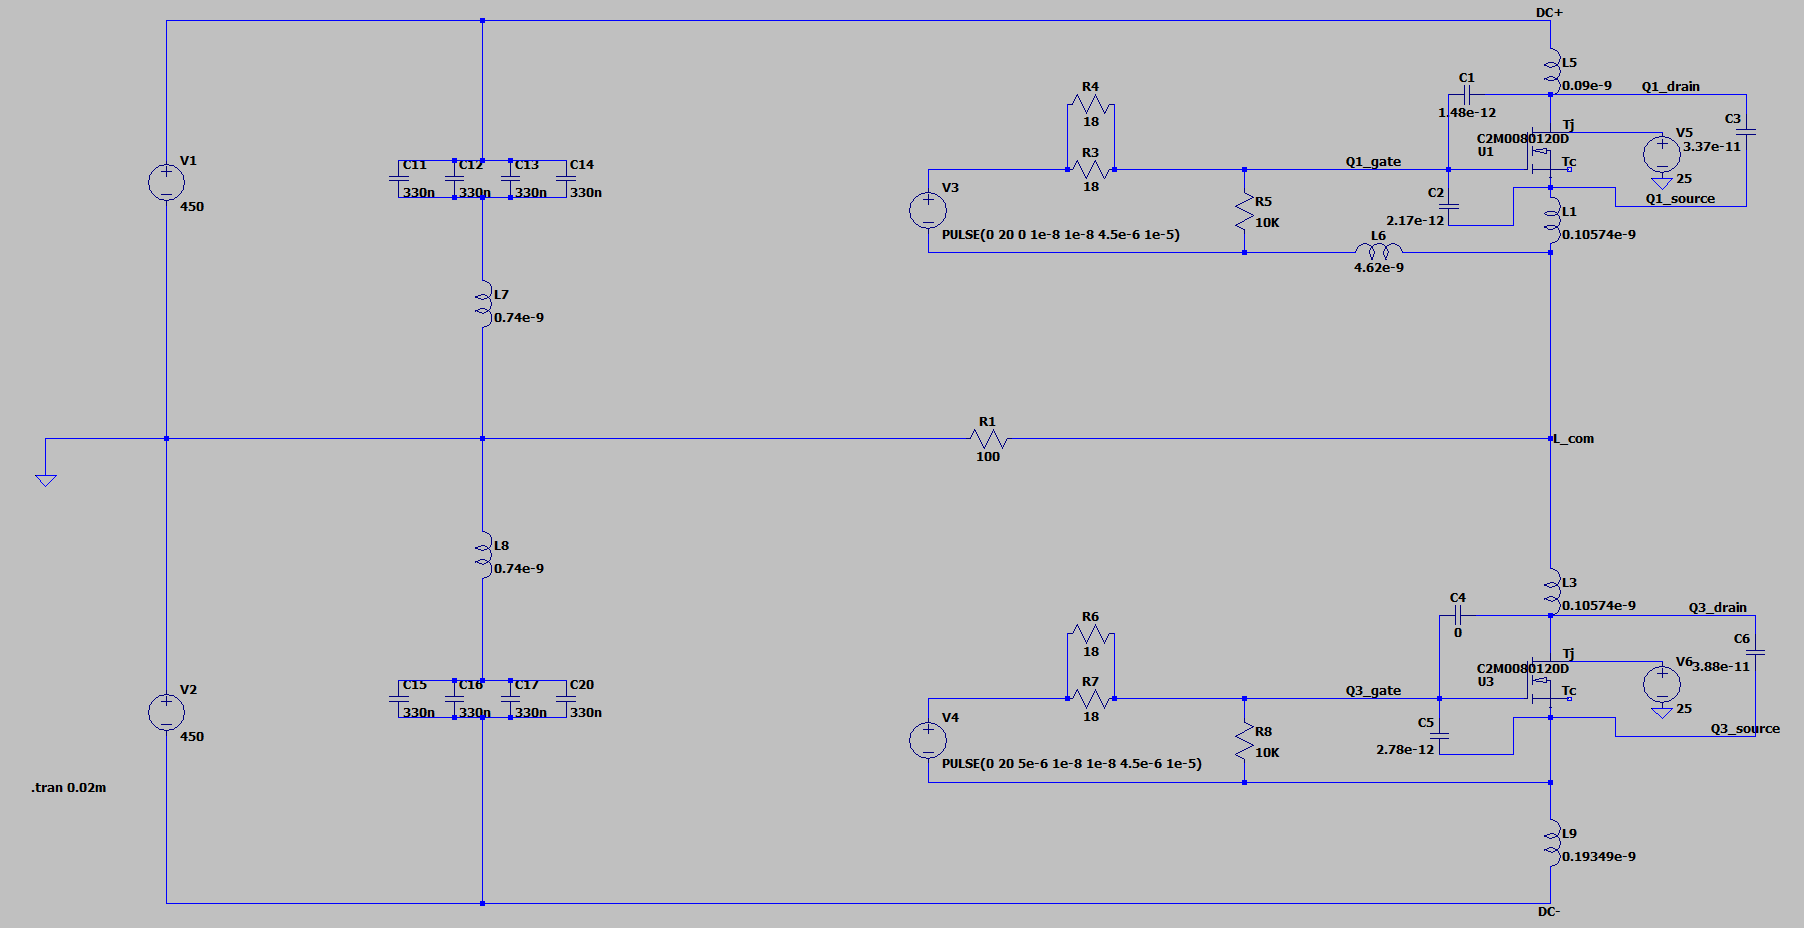
\includegraphics[width=\textwidth]{pictures/implementation/cap/spice_cap_1.PNG}
	\caption{Spice model with capacitances}
	\label{fig:spice_cap}
\end{figure}

\subsubsection{Q1 gate and drain}
\label{sec:q1_gate_drain}

The capacitance was extracted between the nets seen in Figure \ref{fig:cap_q1_g_d}. Its value of $1.48 pF$ is in the expected order of magnitude.

\begin{figure}[H]
	\centering
	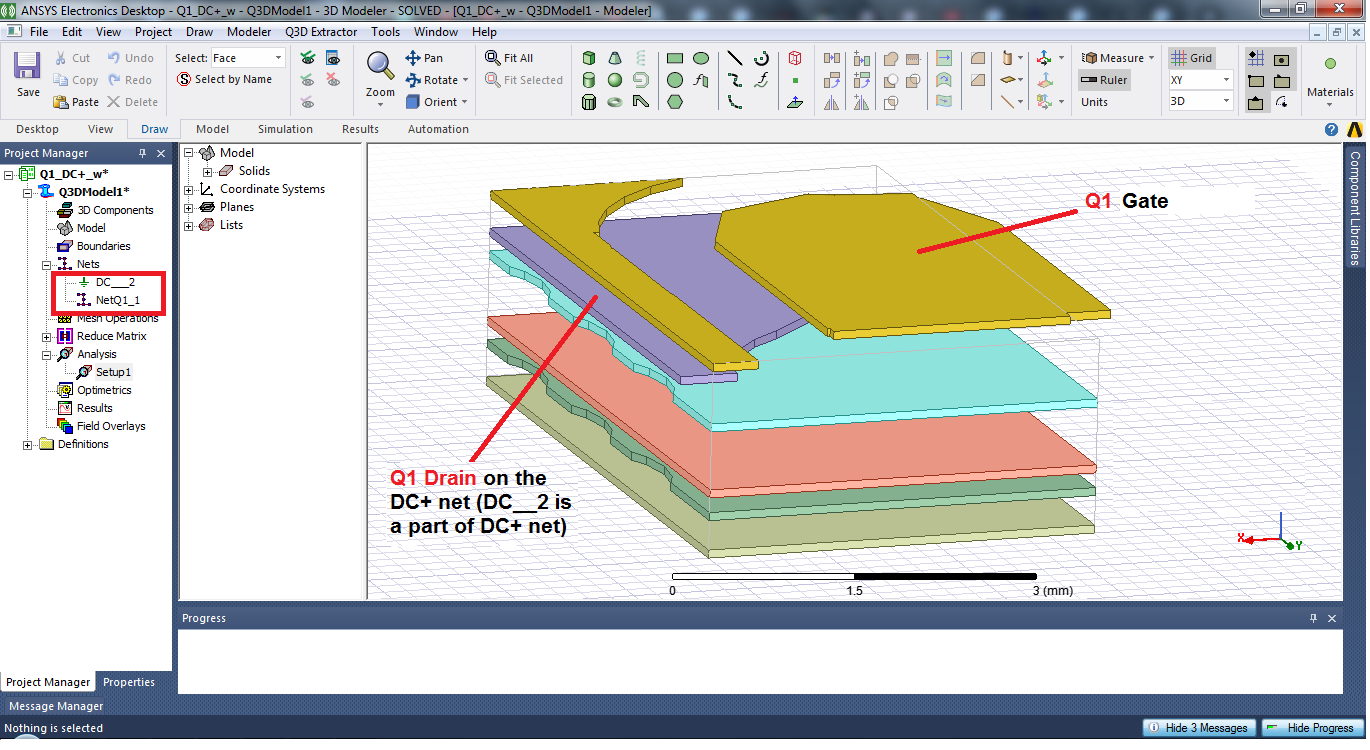
\includegraphics[width=\textwidth]{pictures/implementation/cap/cap_q1_g_d.PNG}
	\caption{The Q1-gate and Q1-drain net}
	\label{fig:cap_q1_g_d}
\end{figure}

\subsubsection{Q1 gate and source}
\label{sec:q1_gate_source}

The capacitance was extracted between the nets seen in Figure \ref{fig:cap_q1_g_s}. Its value of $2.17 pF$ is in the expected order of magnitude.

\begin{figure}[H]
	\centering
	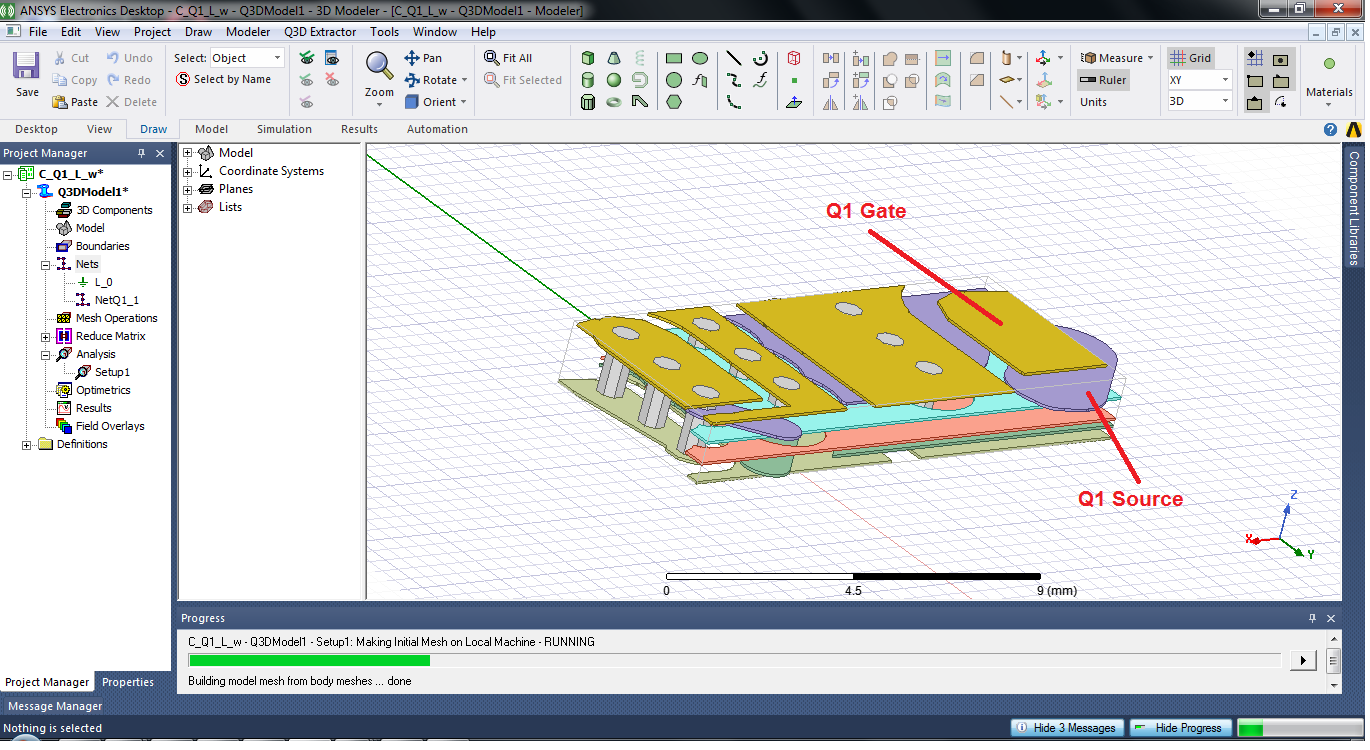
\includegraphics[width=\textwidth]{pictures/implementation/cap/cap_q1_g_s.PNG}
	\caption{The Q1-gate and Q1-source net}
	\label{fig:cap_q1_g_s}
\end{figure}

\subsubsection{Q1 drain and source}
\label{sec:q1_drain_source}

The capacitance was extracted between the nets seen in Figure \ref{fig:cap_q1_d_s}. Its value of $33.7 pF$ is in the expected order of magnitude.

\begin{figure}[H]
	\centering
	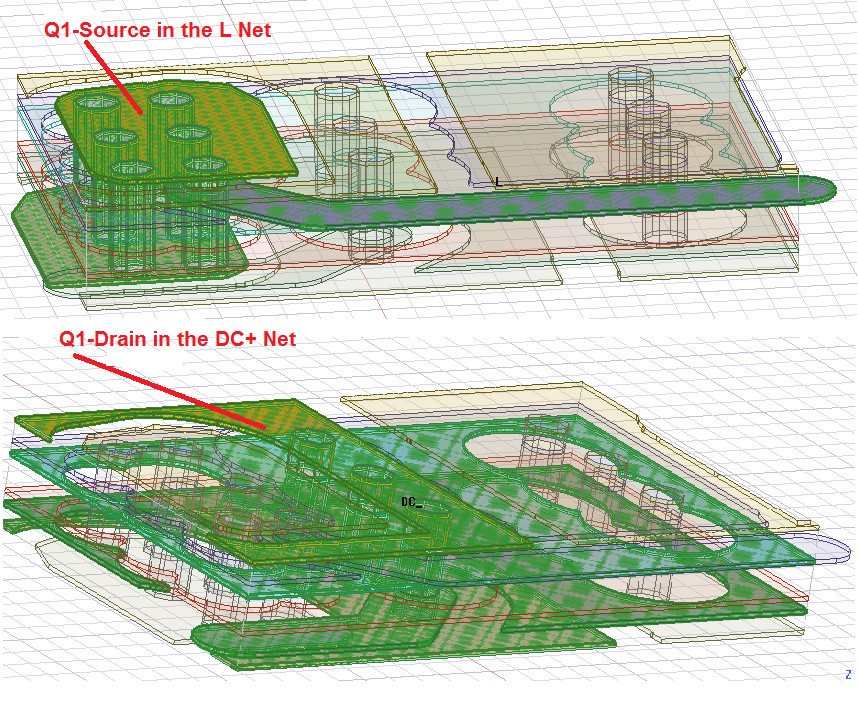
\includegraphics[width=\textwidth]{pictures/implementation/cap/cap_q1_d_s.PNG}
	\caption{The Q1-drain and Q1-source net}
	\label{fig:cap_q1_d_s}
\end{figure}

\subsubsection{Q3 gate and drain}
\label{sec:q3_gate_drain}

Capacitance was attempted to be extracted between the nets seen in Figure \ref{fig:cap_q3_g_d}. Since there is no coupling between them, there is no appreciable capacitance.

\begin{figure}[H]
	\centering
	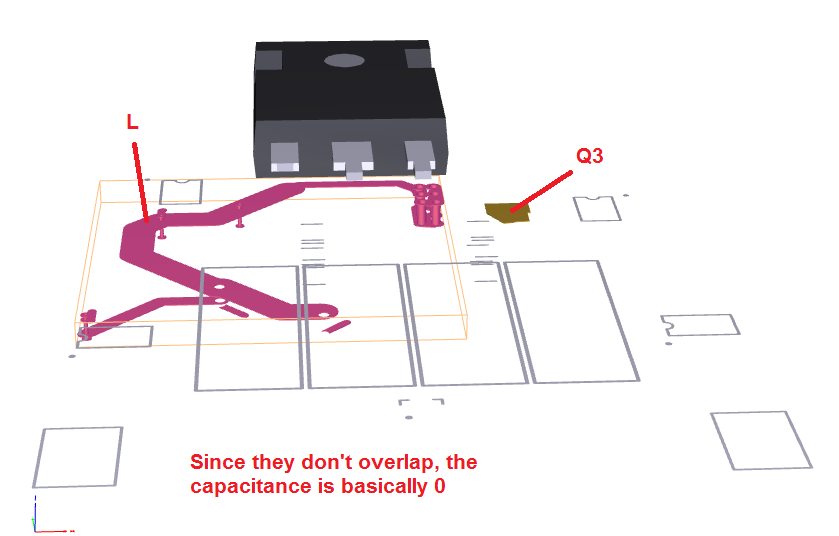
\includegraphics[width=\textwidth]{pictures/implementation/cap/cap_q3_g_d.PNG}
	\caption{The Q3-gate and Q3-drain net}
	\label{fig:cap_q3_g_d}
\end{figure}

\subsubsection{Q3 gate and source}
\label{sec:q3_gate_source}

The capacitance was extracted between the nets seen in Figure \ref{fig:cap_q3_g_s}. Its value of $2.78 pF$ is in the expected order of magnitude.

\begin{figure}[H]
	\centering
	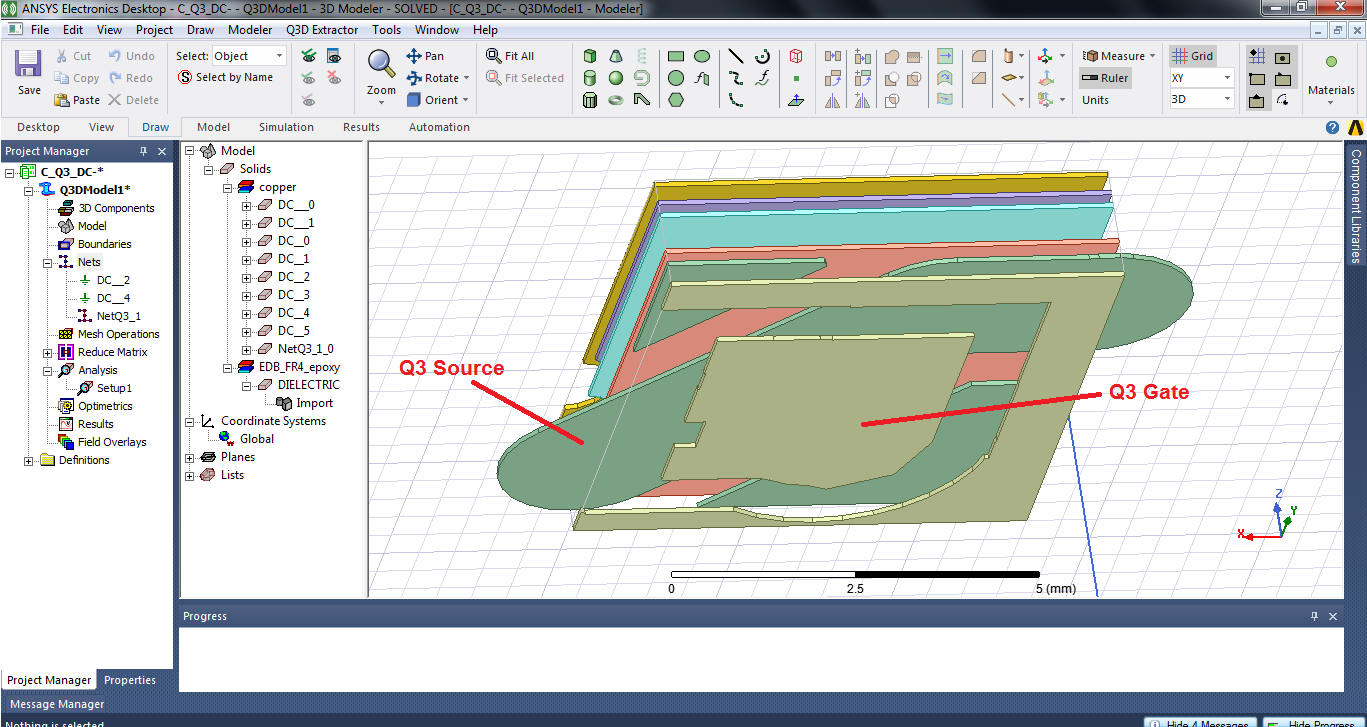
\includegraphics[width=\textwidth]{pictures/implementation/cap/cap_q3_g_s.PNG}
	\caption{The Q3-gate and Q3-source net}
	\label{fig:cap_q3_g_s}
\end{figure}

\subsubsection{Q3 drain and source}
\label{sec:q3_drain_source}

The capacitance was extracted between the nets seen in Figure \ref{fig:cap_q3_d_s}. Its value of $38.8 pF$ is in the expected order of magnitude.

\begin{figure}[H]
	\centering
	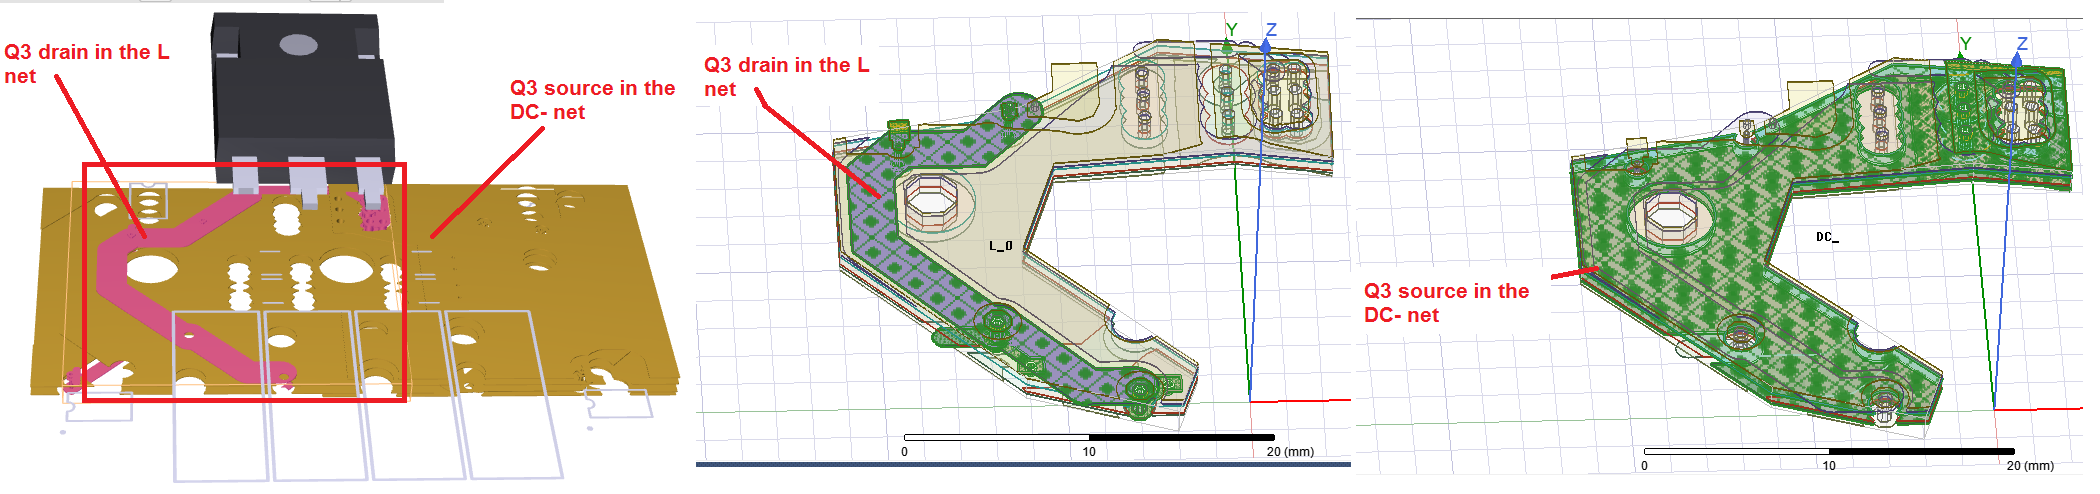
\includegraphics[width=\textwidth]{pictures/implementation/cap/cap_q3_d_s.PNG}
	\caption{The Q3-drain and Q3-source net}
	\label{fig:cap_q3_d_s}
\end{figure}


\subsubsection{Waveforms}
\label{sec:cap_waveforms}

The simulated waveforms look plausible. Some cross-coupling can be seen at the moment of the switching but this is not enough to trigger false turn on-off cycles.

Figure \ref{fig:cap_gates_1} shows two whole cycles as an overview, Figure \ref{fig:cap_gates_2} shows the transient where $V_{GS1}$ turns off, Figure \ref{fig:cap_gates_3} depicts the other end of that cycle. Figure \ref{fig:cap_load} demonstrates the voltage and current of the load.

\begin{figure}[H]
	\centering
	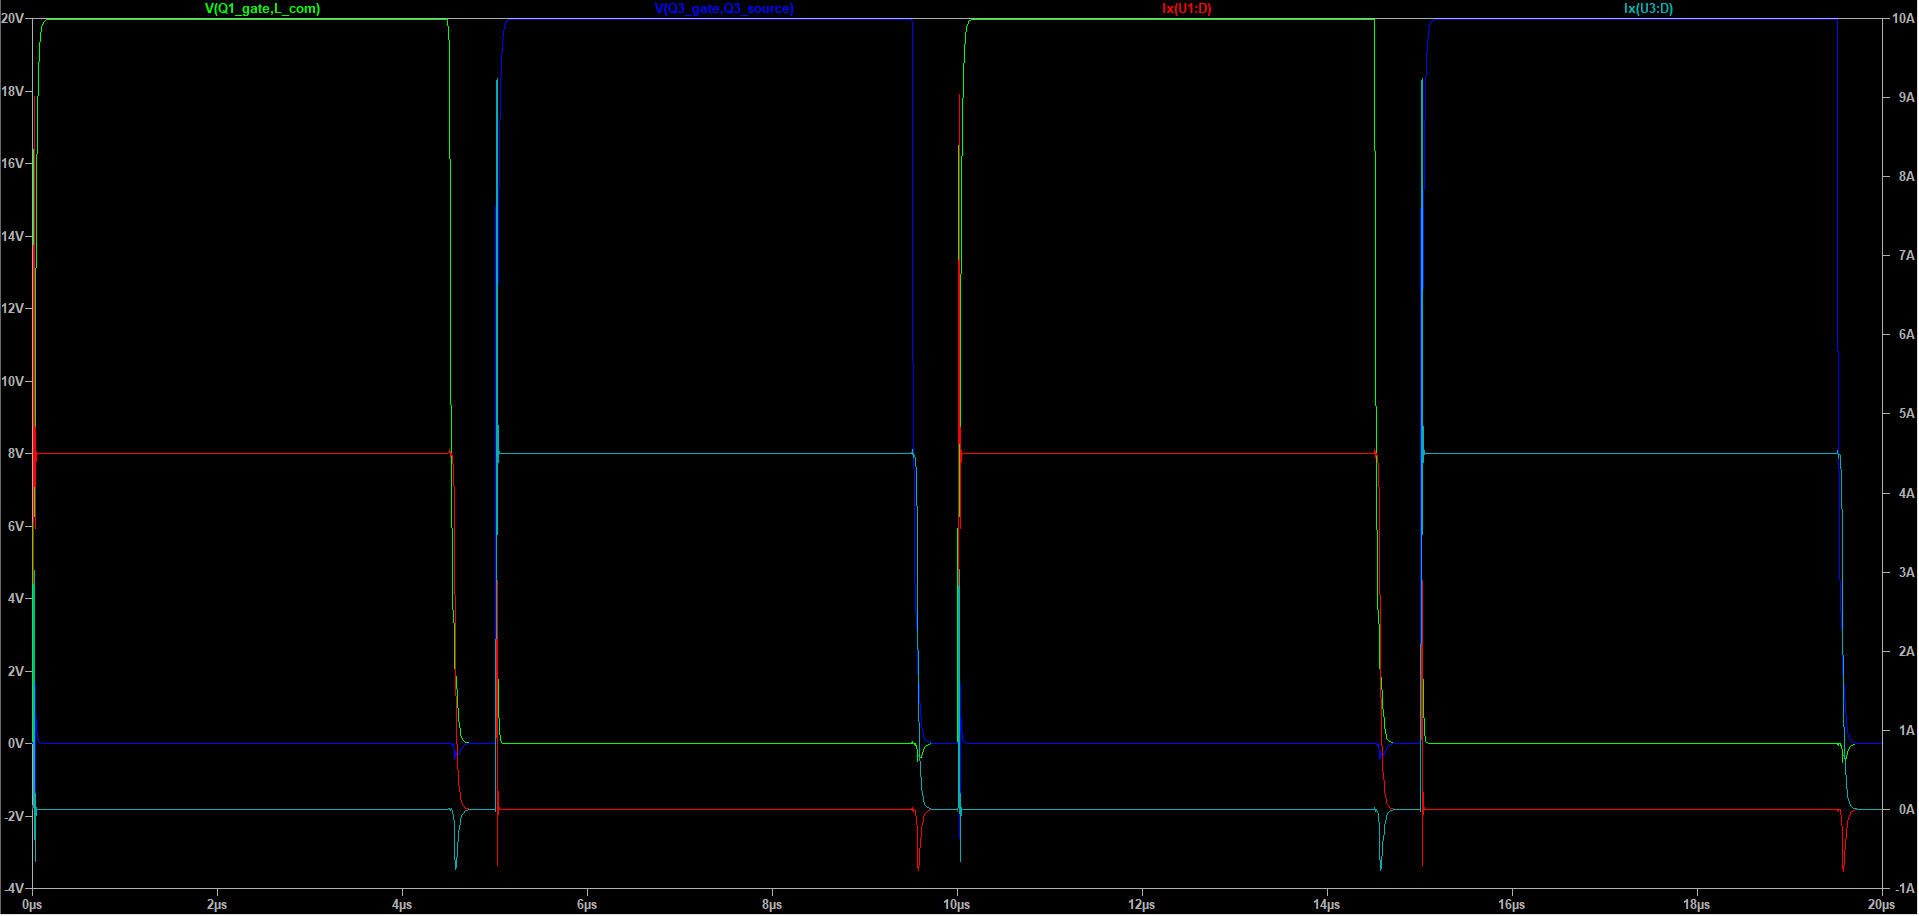
\includegraphics[width=\textwidth]{pictures/implementation/cap/cap_gates_1.PNG}
	\caption{Overview of the gate voltages and drain currents}
	\label{fig:cap_gates_1}
\end{figure}

\begin{figure}[H]
	\centering
	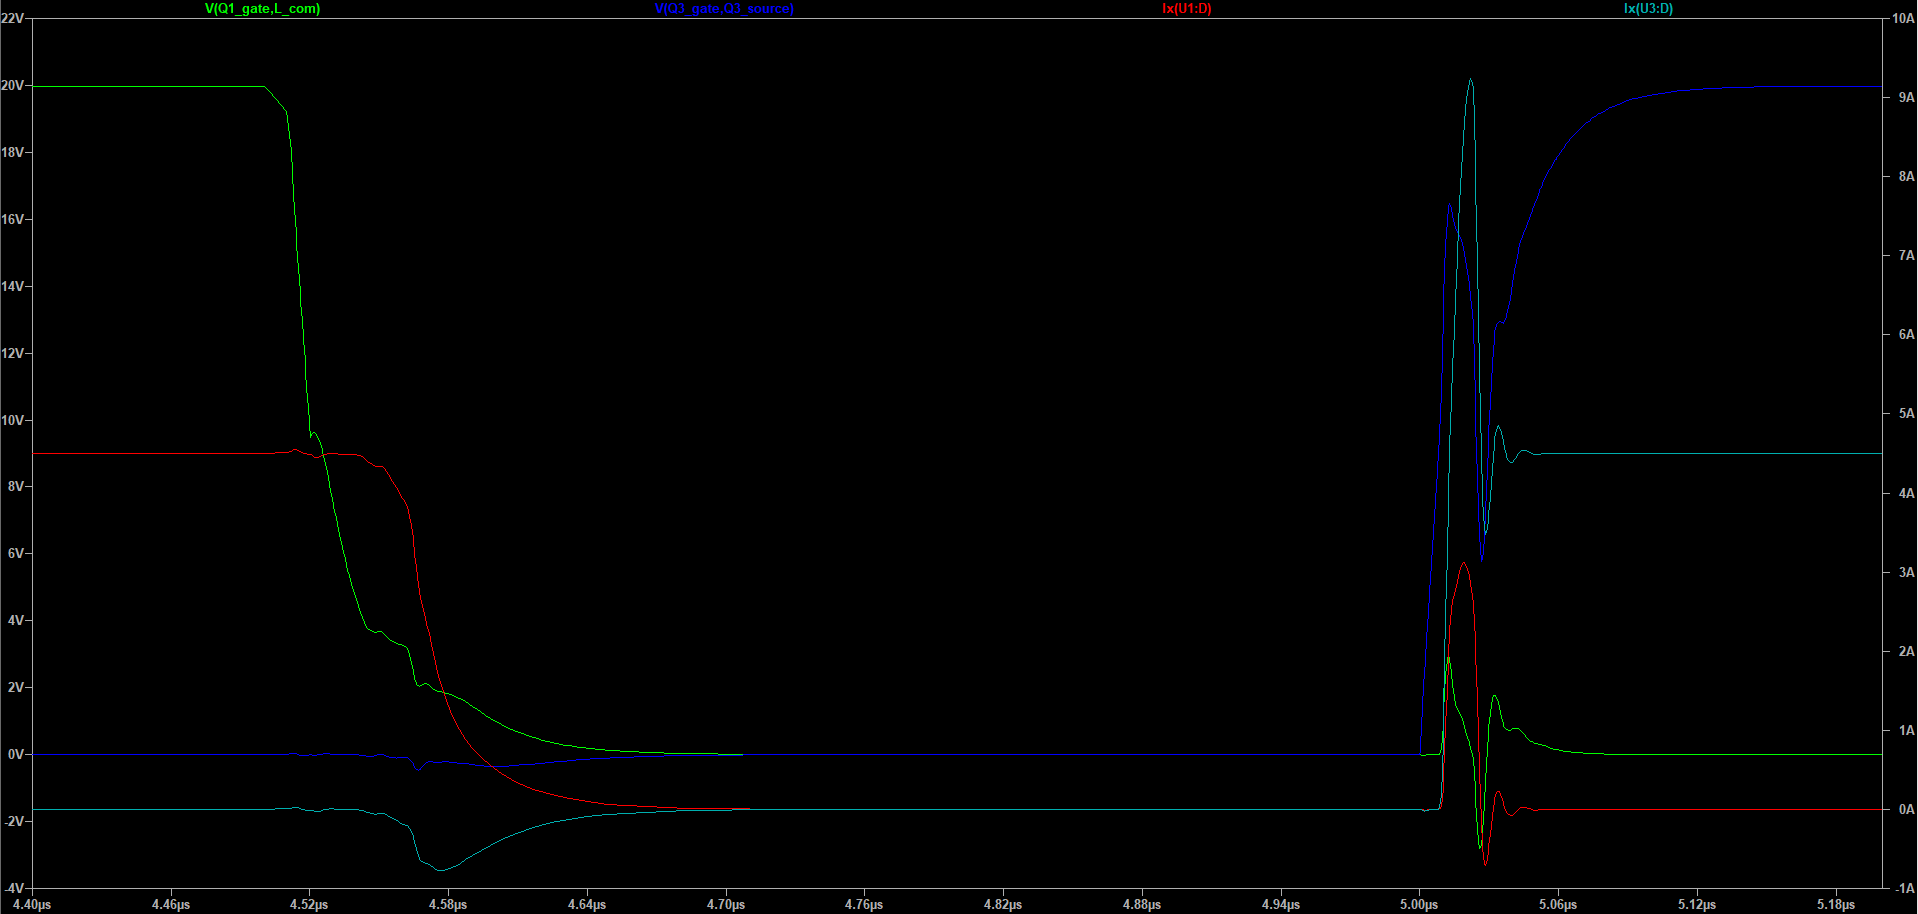
\includegraphics[width=\textwidth]{pictures/implementation/cap/cap_gates_2.PNG}
	\caption{Q1 turn off transient, gate voltages and drain currents}
	\label{fig:cap_gates_2}
\end{figure}

\begin{figure}[H]
	\centering
	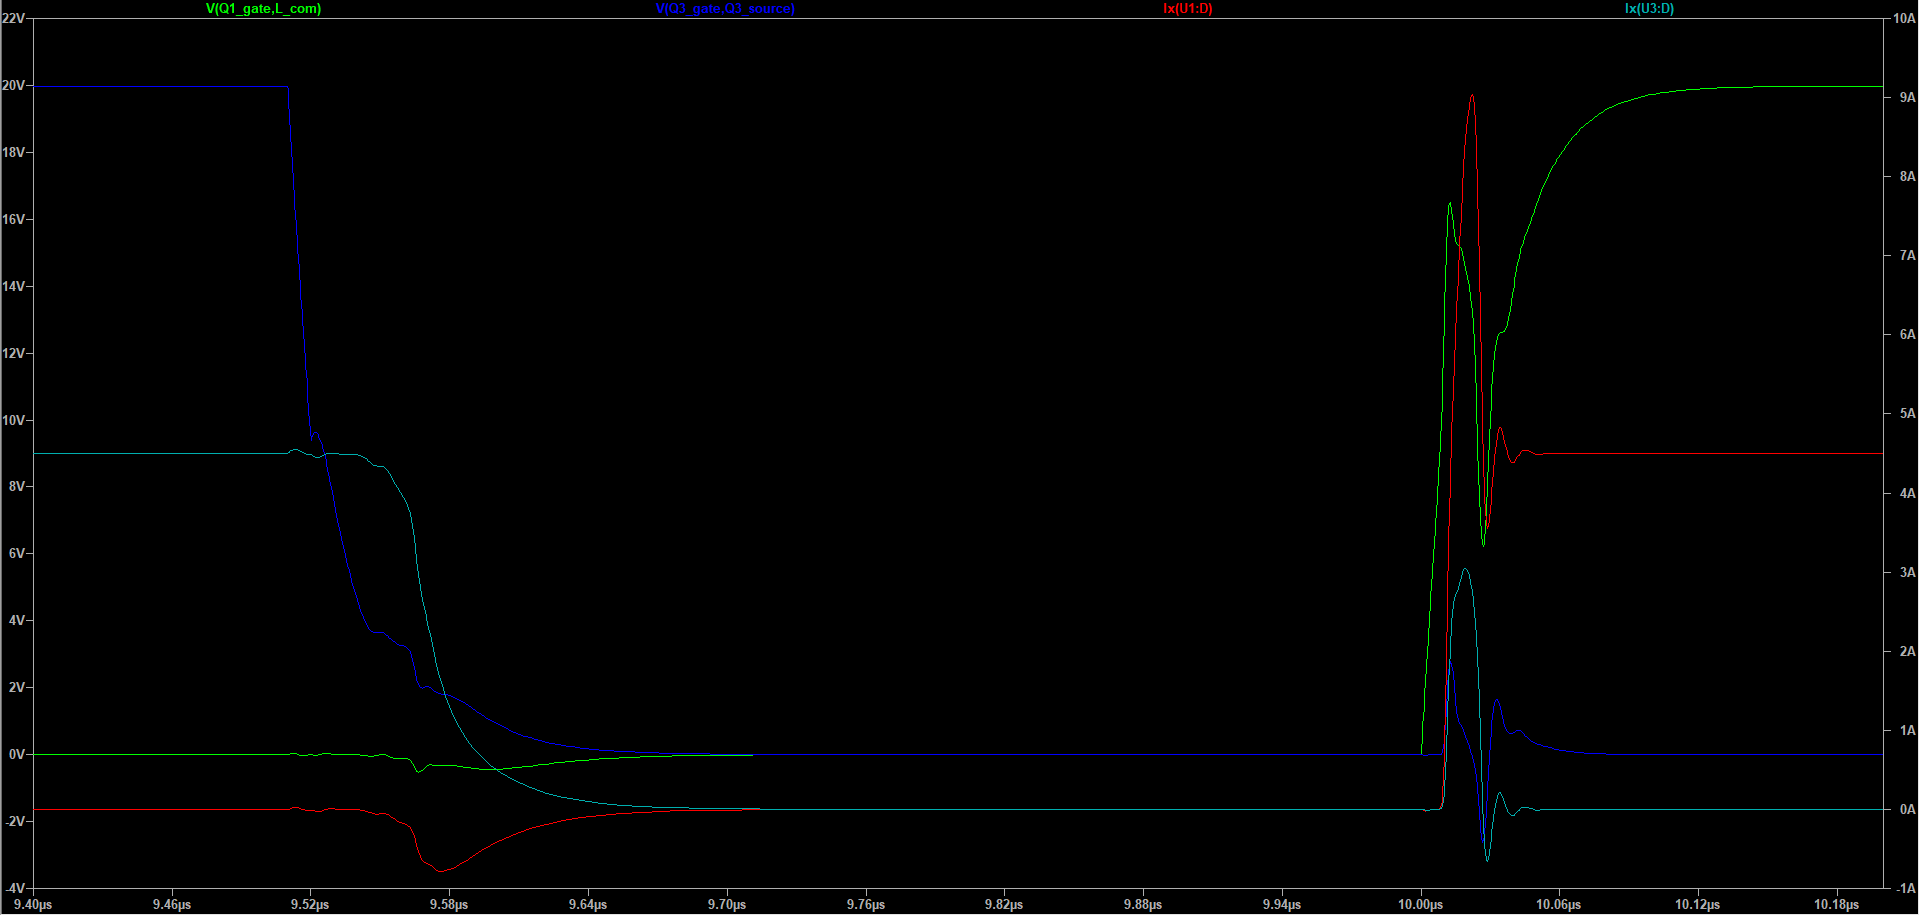
\includegraphics[width=\textwidth]{pictures/implementation/cap/cap_gates_3.PNG}
	\caption{Q3 turn off transient, gate voltages and drain currents}
	\label{fig:cap_gates_3}
\end{figure}

\begin{figure}[H]
	\centering
	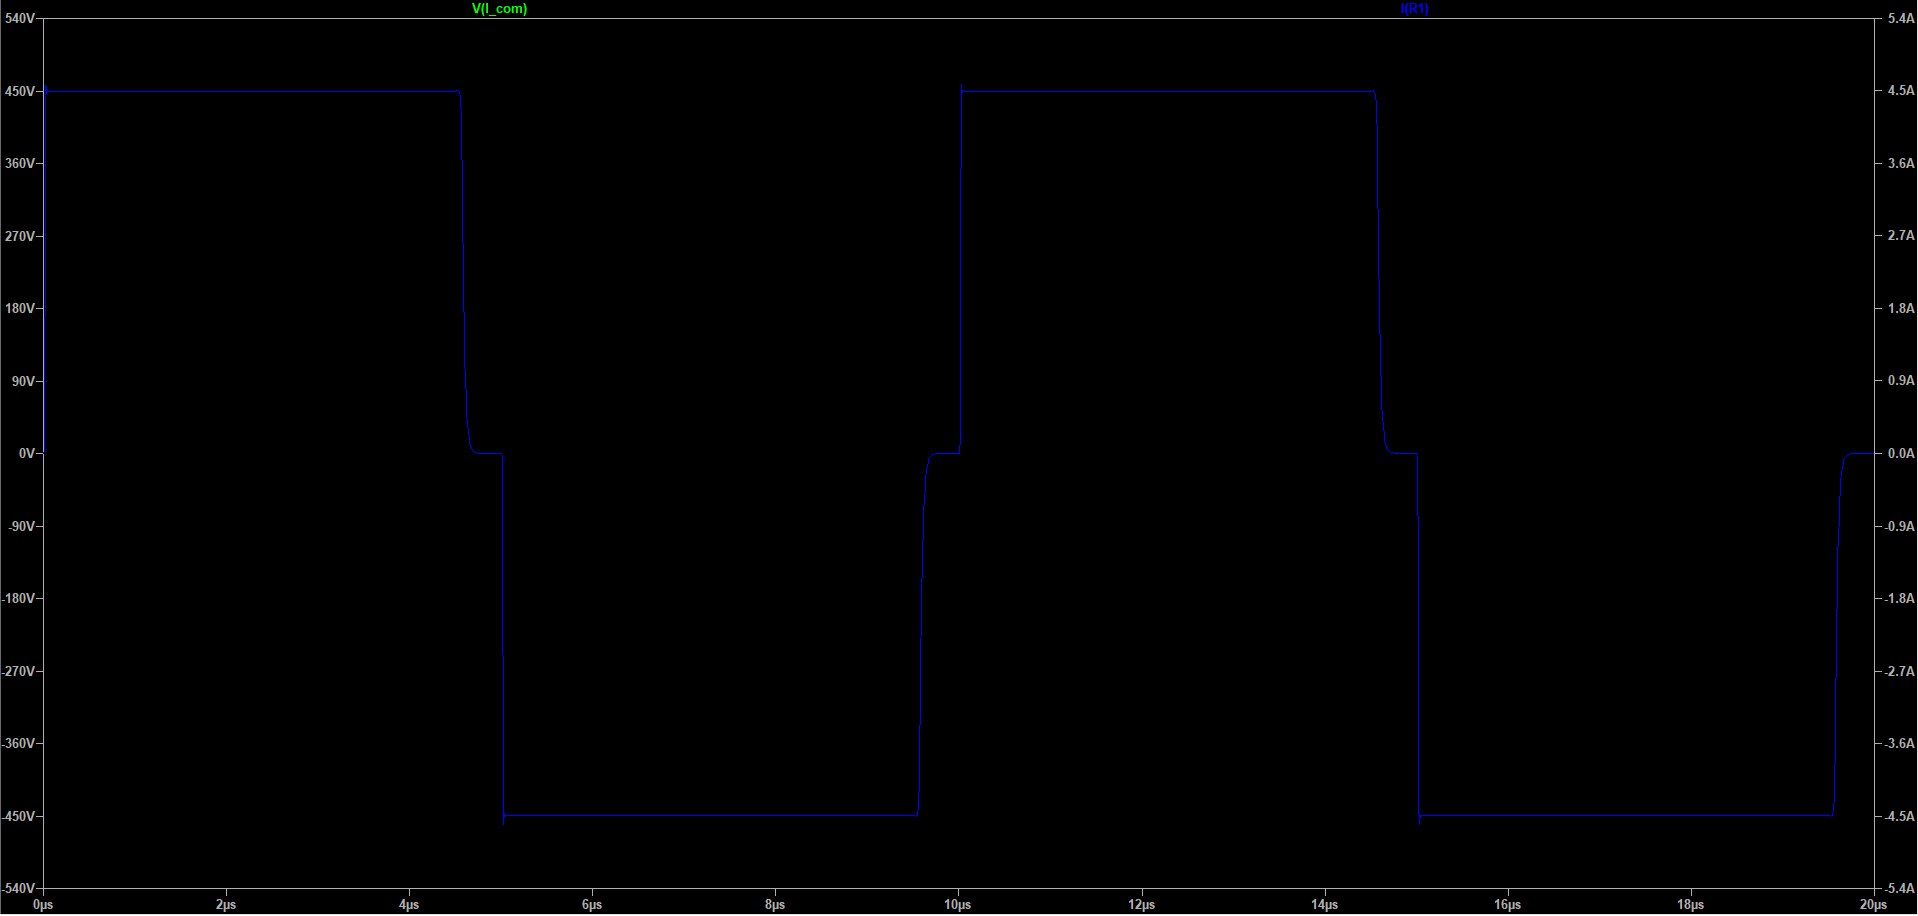
\includegraphics[width=\textwidth]{pictures/implementation/cap/cap_load.PNG}
	\caption{Voltage and current waveforms of the resistor overlap}
	\label{fig:cap_load}
\end{figure}